\newpage
\hypertarget{sec:extendGui}{}
\section{Running the Leitner's Box GUI}
\genHeader

In addition to \texttt{removeCard}, the GUI is able to access and execute the \texttt{check} method based on your SDM implementation! First, double check that
your metamodel is saved and built, then run the GUI! 

\begin{itemize}
\item[$\blacktriangleright$] Pick a card from any of your partitions, then run \texttt{check}. You'll be promoted with a dialogue box to make your guess in
(Fig.~\ref{fig:checkGuess}).

\begin{figure}[htp]
\begin{center}
  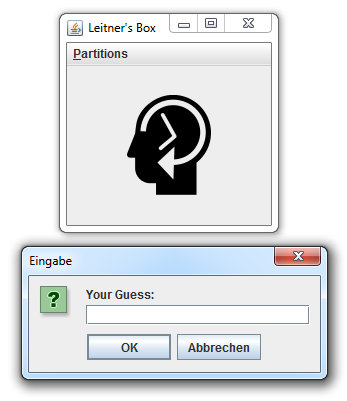
\includegraphics[width=0.5\textwidth]{eclipse_checkGuess}
  \caption{Enter your guess}
  \label{fig:checkGuess}
\end{center}
\end{figure}

\item[$\blacktriangleright$] Enter your word, then press \texttt{OK}. You should immediately see any movemement changes in the drop-down menus, and shortly in
\texttt{box.xmi} after refreshing.

\item[$\blacktriangleright$] Fully test your implementation by making right and wrong guesses. Watch how they cards move around -- do they
behave as expected, by the rules of Leitner Box?

\item[$\blacktriangleright$] At this point, we invite you to browse the \texttt{LeitnersBoxController.java} file. Can you see how \texttt{removeCard} and
\texttt{check} were called and executed? You are encouraged to modify this file so that you may be able to test future SDM implementations.

\end{itemize}
